% Stunde 1 — Inhaltsblatt
% Kompilieren mit: lualatex inhalt.tex
\documentclass[11pt,a4paper,DIV=12]{scrartcl}

\usepackage[ngerman]{babel}
\usepackage[haranoaji]{luatexja-preset}
\usepackage{luatexja-ruby}
\usepackage{booktabs}
\usepackage{array}
\usepackage{xcolor}
\usepackage[most]{tcolorbox}
\usepackage{enumitem}
\usepackage{microtype}
\usepackage{graphicx}
\usepackage{wrapfig}
\graphicspath{{../../bilder/}}

\definecolor{akzent}{HTML}{1F4E79}
\definecolor{implizit}{HTML}{1B7A43}
\definecolor{explizit}{HTML}{B3541E}
\definecolor{hell}{HTML}{F4F6F8}

\addtokomafont{disposition}{\color{akzent}}
\setkomafont{title}{\color{akzent}\bfseries}

% Kurzbefehle
\newcommand{\impl}{\textcolor{implizit}{\textbf{implizit}}}
\newcommand{\expl}{\textcolor{explizit}{\textbf{explizit}}}
\newcommand{\jterm}[2]{\ruby{#1}{#2}}
% Deutsche Anfuehrungszeichen: babel-Befehle statt Unicode,
% sonst haelt luatexja sie fuer Japanisch und setzt Abstand drumrum.
\newcommand{\zitat}[1]{\glqq #1\grqq{}}

\newtcolorbox{merke}[1][]{
  enhanced, colback=hell, colframe=akzent,
  boxrule=0pt, leftrule=3pt, arc=0pt, outer arc=0pt,
  left=8pt, right=8pt, top=6pt, bottom=6pt,
  #1
}

\title{Stunde 1 — Nomen, Adjektive, Verben}
\subtitle{Implizit oder explizit}
\date{}
\author{}

\begin{document}
\maketitle
\vspace{-2.5em}

\section*{Die Idee: implizit oder explizit}

\textbf{Jedes Wort braucht eine Endung, um sich an ein Nomen zu hängen.}
Der einzige Unterschied ist, ob sie schon drinsteckt.

\begin{center}
\begin{tabular}{@{}llll@{}}
\toprule
 & \textbf{am Nomen} & \textbf{Endung} & \\
\midrule
出る & 出る人 & る & \impl{} — schon im Wort \\
大きい & 大きい犬 & い & \impl{} — schon im Wort \\
日本 & 日本\textbf{の}本 & の & \expl{} — muss dazu \\
\jterm{大切}{たいせつ} & \jterm{大切}{たいせつ}\textbf{な}本 & な & \expl{} — muss dazu \\
\bottomrule
\end{tabular}
\end{center}

Verben und い-Adjektive tragen ihr Kennzeichen \textbf{eingebaut}. Nomen und
な-Adjektive stehen nackt da und müssen es sich \textbf{anbauen}.

\begin{merke}
Das ist die ganze Stunde. Alles Weitere ist dieselbe Regel nochmal.
\end{merke}

\section{Am Nomen (attributiv)}

\textbf{Attributiv} heißt: das Wort hängt an einem Nomen und beschreibt es.

\begin{center}
\begin{tabular}{@{}ll@{}}
大きい犬 & attributiv (beschreibt den Hund) \\
犬、大きい。& prädikativ (ist die Aussage) \\
\end{tabular}
\end{center}

\begin{center}
\begin{tabular}{@{}lll>{\quad}l@{}}
\toprule
\impl{} & Verb & 出る人 & る macht's \\
\impl{} & い-Adj & 大きい犬 & い macht's \\
\expl{} & Nomen & 日本\textbf{の}本 & の dazu \\
\expl{} & な-Adj & \jterm{大切}{たいせつ}\textbf{な}本 & な dazu \\
\bottomrule
\end{tabular}
\end{center}

\section{Als Aussage (prädikativ)}

Dieselbe Regel, zweiter Durchgang:

\begin{center}
\begin{tabular}{@{}lll>{\quad}l@{}}
\toprule
\impl{} & Verb & 出る。& fertig — る macht's \\
\impl{} & い-Adj & 大きい。& fertig — い macht's \\
\expl{} & Nomen & 日本\textbf{だ}。& だ dazu \\
\expl{} & な-Adj & \jterm{大切}{たいせつ}\textbf{だ}。& だ dazu \\
\bottomrule
\end{tabular}
\end{center}

Das angebaute Ding zum Behaupten heißt \textbf{だ}.

\begin{merke}
\textbf{Kleine Feinheit:} Bei な-Adjektiven ist das Angebaute \emph{beide Male
dasselbe} — な \emph{ist} だ, nur attributiv. \jterm{大切}{たいせつ}な\,/\,\jterm{大切}{たいせつ}だ
= ein Ding, zwei Formen.\\
Bei Nomen sind es \emph{zwei verschiedene} Teile: の zum Anhängen, だ zum Behaupten.
な-Adjektive stehen also näher an だ als Nomen.
\end{merke}

\section{Verneinen}

\begin{center}
\begin{tabular}{@{}llll@{}}
\toprule
\impl{} & い-Adj & 大きい → 大き\textbf{くない} & das い wird verneint \\
\impl{} & Verb (る) & 出る → 出\textbf{ない} & る weg, ない dran \\
\impl{} & Verb (う) & 立つ → 立\textbf{た}ない & う-Reihe → あ-Reihe, ない dran \\
\expl{} & Nomen & 犬 → 犬\textbf{じゃない} & das だ wird verneint \\
\expl{} & な-Adj & \jterm{大切}{たいせつ} → \jterm{大切}{たいせつ}\textbf{じゃない} & das だ wird verneint \\
\bottomrule
\end{tabular}
\end{center}

\textbf{Warum ist explizit immer じゃない?} Weil gar nicht das Wort verneint wird,
sondern das angebaute だ — und das ist immer dasselbe, egal ob 犬 oder
\jterm{大切}{たいせつ} davorsteht.

\begin{description}[leftmargin=1.5em,style=nextline,itemsep=2pt]
\item[う-Verben] 立\textbf{つ}→立\textbf{た}ない \quad 正\textbf{す}→正\textbf{さ}ない \quad
  \jterm{引}{ひ}\textbf{く}→\jterm{引}{ひ}\textbf{か}ない \quad 上\textbf{る}→上\textbf{ら}ない
\item[Unregelmäßig] する→しない
\end{description}

\section{Vergangenheit}

\begin{center}
\begin{tabular}{@{}lll>{\quad}l@{}}
\toprule
\impl{} & い-Adj & 大きい → 大き\textbf{かった} & das い wird Vergangenheit \\
\expl{} & Nomen & 犬 → 犬\textbf{だった} & das だ wird Vergangenheit \\
\expl{} & な-Adj & \jterm{大切}{たいせつ} → \jterm{大切}{たいせつ}\textbf{だった} & dito \\
\impl{} & Verb & \textbf{→ nächste Stunde} & \\
\bottomrule
\end{tabular}
\end{center}

Verben lassen wir aus: ihre Vergangenheit braucht \jterm{音便}{おんびん}, den
Lautwandel — \jterm{引}{ひ}く→\jterm{引}{ひ}\textbf{いた}, 立つ→立\textbf{った},
上る→上\textbf{った}. Sechs Muster plus eine Ausnahme. Eigene Stunde.

\section{Die だ-Falle}

だ liegt unter der expliziten Gruppe — aber im blanken Satz \textbf{fällt es weg}:

\begin{center}
\begin{tabular}{@{}ll@{}}
\jterm{大人}{おとな}だ。& → klingt schroff \\
\jterm{大人}{おとな}。& → so redet man wirklich \\
\end{tabular}
\end{center}

Es taucht auf, sobald etwas dranhängt: \jterm{大人}{おとな}\textbf{だ}よ。\,/\,
\jterm{大人}{おとな}\textbf{だ}ね。\,/\, \jterm{大人}{おとな}\textbf{だ}から、…

In じゃない und だった steckt es sowieso schon drin.

\begin{merke}
だ ist nicht optional. Es ist \textbf{die Form unter allem}, nur meistens unsichtbar.
\end{merke}

\section{Wie man antwortet}

\begin{wrapfigure}{l}{3.6cm}
  \vspace{-1.2\baselineskip}
  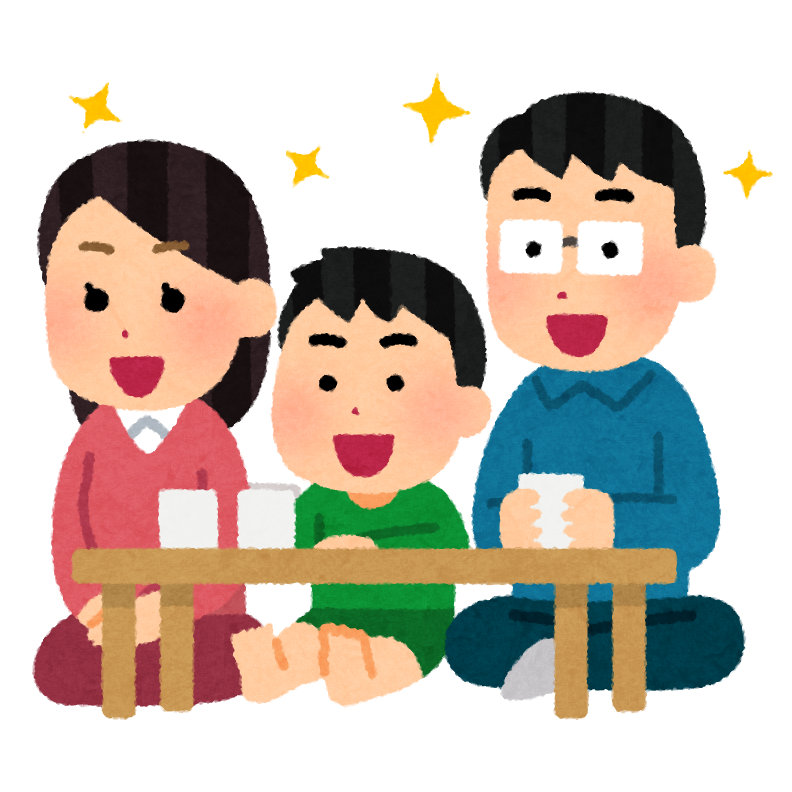
\includegraphics[width=3.4cm]{ochanoma_happy_notv.png}
  \vspace{-1.2\baselineskip}
\end{wrapfigure}
Auf eine Ja/Nein-Frage antwortet man im Japanischen oft \textbf{gar nicht mit \zitat{ja}
oder \zitat{nein}}, sondern man \textbf{wiederholt das Prädikat}:

\begin{center}
\begin{tabular}{@{}ll@{}}
立つ？ & → 立たない。\\
犬？ & → 犬じゃない。\jterm{牛}{うし}。\\
大きい？ & → 大きい。\\
\end{tabular}
\end{center}

Das ist keine Notlösung, sondern das Übliche. Fragen geht genauso: \textbf{einfach
die Stimme heben.} Es braucht kein Fragewort und kein か.

\begin{merke}
ええ (ja) haben wir schon. うん\,/\,ううん — die lockeren Varianten — kommen in ein
paar Stunden dazu, wenn dein WaniKani-Level soweit ist. Bis dahin: Prädikat
wiederholen. Ist ohnehin japanischer.
\end{merke}

\section{Warum das so ist — ein bisschen Geschichte}

Die Einteilung ist kein Zufall und keine Schikane. Sie ist ein \textbf{Unfall der
Sprachgeschichte}.

Im klassischen Japanisch hatten \emph{alle} Wortarten zwei getrennte Formen — eine
fürs Satzende, eine fürs Anhängen ans Nomen:

\begin{center}
\begin{tabular}{@{}lll@{}}
\toprule
 & \textbf{Satzende} (\jterm{終止形}{しゅうしけい}) & \textbf{am Nomen} (\jterm{連体形}{れんたいけい}) \\
\midrule
Verb & \jterm{出}{い}づ & \jterm{出}{い}づ\textbf{る} \\
い-Adj & \jterm{正}{ただ}\textbf{し} & \jterm{正}{ただ}し\textbf{き} \\
Kopula & な\textbf{り} & な\textbf{る} \\
\bottomrule
\end{tabular}
\end{center}

Dann sind bei \textbf{Verben und い-Adjektiven die beiden zusammengefallen}:
出づる → 出る, 正しき → 正しい. Heute sieht man da keinen Unterschied mehr, weil keiner
mehr da ist. Die Form \emph{ist} beides.

\textbf{Bei der Kopula ist das nie passiert.} な (am Nomen) und だ (am Satzende) sind
getrennt geblieben.

\begin{merke}
\textbf{Das ist die Antwort auf \zitat{warum diese zwei Gruppen}:} Nicht weil Nomen
irgendwie defizitär wären — sondern weil bei der einen Gruppe zwei Formen
verschmolzen sind und bei der anderen nicht.\\[4pt]
\zitat{Implizit} ist ein historischer Zusammenfall. \zitat{Explizit} ist der Rest, der sich
geweigert hat.
\end{merke}

Der Begriff \jterm{連体形}{れんたいけい} sagt das übrigens wörtlich: 連 \zitat{verbinden}
+ 体 (wie in \jterm{体言}{たいげん} = Nomen) + 形 \zitat{Form} → \textbf{\zitat{die Form, mit der
man sich an ein Nomen anschließt.}} Die Japaner haben für genau das, worum es hier
geht, ein eigenes Wort.

\section{Wie Japaner das selbst einteilen}

Wichtig zu wissen, weil du das früher oder später liest — und weil es \textbf{anders}
ist als unsere Einteilung.

Im \jterm{国文法}{こくぶんぽう}, der Schulgrammatik japanischer Mittelstufenschüler:

\begin{center}
\begin{tabular}{@{}ll@{}}
\jterm{体言}{たいげん} & = nur Nomen \\
\jterm{用言}{ようげん} & = Verben, い-Adjektive \textbf{und な-Adjektive} \\
\end{tabular}
\end{center}

な-Adjektive stehen dort also \textbf{bei den Verben}, nicht bei den Nomen — genau
andersrum als bei uns. Sie heißen dort \jterm{形容動詞}{けいようどうし}, wörtlich
\zitat{Adjektiv-\textbf{verb}}, und gelten als \emph{ein} Wort, das selbst konjugiert:

\begin{center}
\jterm{大切}{たいせつ}だろ・\jterm{大切}{たいせつ}だっ・\jterm{大切}{たいせつ}で・%
\jterm{大切}{たいせつ}に・\jterm{大切}{たいせつ}だ・\jterm{大切}{たいせつ}\textbf{な}・%
\jterm{大切}{たいせつ}なら
\end{center}

Das な in \jterm{大切}{たいせつ}な本 ist dort das \jterm{連体形}{れんたいけい} dieses
Wortes — nicht \zitat{だ attributiv}. Und 日本だ ist dort etwas ganz anderes, nämlich Nomen
+ Hilfsverb. \textbf{国文法 sagt ausdrücklich: 日本だ und \jterm{大切}{たいせつ}だ sind
nicht dasselbe.}

Wir behaupten das Gegenteil. Warum?

Weil 国文法 dafür gebaut ist, \textbf{klassische Texte zu lesen} — daher die
Konjugationstabellen oben. Unsere Version erklärt mit \emph{einer} Regel, warum
犬じゃない und \jterm{大切}{たいせつ}じゃない identisch aussehen. 国文法 muss das als
Zufall behandeln: zwei Strukturen, gleiches Ergebnis.

\begin{merke}
\textbf{Beide beschreiben dieselben Sätze richtig. Sie zerlegen sie nur anders.}
Keine ist falsch — es sind zwei Werkzeuge für zwei Zwecke.
\end{merke}

\begin{wrapfigure}{r}{3.6cm}
  \vspace{-1.2\baselineskip}
  
\includegraphics[width=3.4cm]{eto_centaur_happy.png}
  \vspace{-1.2\baselineskip}
\end{wrapfigure}
Interessant: Der Name \jterm{形容動詞}{けいようどうし} gibt uns halb recht.
\zitat{Adjektiv-\emph{verb}} heißt ja gerade, dass sie sich verbhaft verhalten — weil das
だ drinsteckt und konjugiert. Wir sagen: das だ ist ein eigenes Teil. 国文法 sagt: es
gehört zum Wort. Denselben Sachverhalt sehen beide.

\section*{Vokabeln}

Alles aus WaniKani Level 1–3. \textbf{Level 1–2 ohne Furigana, Level 3 mit} — die
hast du gerade erst.

\begin{description}[leftmargin=0pt,style=nextline,itemsep=4pt]

\item[Nomen]
人 Mensch \textbullet{} 犬 Hund \textbullet{} 本 Buch \textbullet{} 水 Wasser \textbullet{}
子 Kind \textbullet{} 日本 Japan \textbullet{} 山 Berg \textbullet{} 川 Fluss \textbullet{}
目 Auge \textbullet{} 手 Hand \textbullet{} 木 Baum \textbullet{} 火 Feuer \textbullet{}
\jterm{大人}{おとな} Erwachsener \textbullet{} 天才 Genie \textbullet{} 女の子 Mädchen \textbullet{}
白人 Weißer \textbullet{} \jterm{父}{ちち} Vater \textbullet{} お\jterm{父}{とう}さん Vater (höfl.) \textbullet{}
\jterm{母}{はは} Mutter \textbullet{} お\jterm{母}{かあ}さん Mutter (höfl.) \textbullet{}
\jterm{牛}{うし} Kuh \textbullet{} \jterm{友人}{ゆうじん} Freund \textbullet{}
\jterm{字}{じ} Schriftzeichen \textbullet{} \jterm{心}{こころ} Herz \textbullet{}
\jterm{今}{いま} jetzt \textbullet{} \jterm{外}{そと} draußen \textbullet{}
\jterm{外人}{がいじん} Ausländer \textbullet{} \jterm{アメリカ人}{あめりかじん} \textbullet{}
\jterm{イギリス人}{いぎりすじん} \textbullet{} \jterm{フランス人}{ふらんすじん} \textbullet{}
リンゴ Apfel \textbullet{} コーヒー Kaffee

\item[な-Adjektive]
上手 gut (in etwas) \textbullet{} 下手 schlecht (in etwas) \textbullet{}
\jterm{大切}{たいせつ} wichtig

\item[い-Adjektive]
大きい groß \textbullet{} 小さい klein \textbullet{} 丸い rund \textbullet{}
正しい richtig \textbullet{} \jterm{古}{ふる}い alt \textbullet{} \jterm{広}{ひろ}い weit \textbullet{}
\jterm{太}{ふと}い dick \textbullet{} \jterm{少}{すく}ない wenig

\item[る-Verben]
出る rausgehen \textbullet{} 上げる hochheben \textbullet{} 下げる runterlassen \textbullet{}
\jterm{止}{と}める anhalten \textbullet{} \jterm{広}{ひろ}げる ausbreiten

\item[う-Verben]
立つ stehen \textbullet{} 正す berichtigen \textbullet{} 上る hochsteigen \textbullet{}
\jterm{引}{ひ}く ziehen

\item[Unregelmäßig]
する machen

\item[Kleinkram]
これ das hier \textbullet{} ええ ja \textbullet{} いつ wann \textbullet{}
\jterm{少}{すこ}し ein bisschen

\end{description}

\end{document}
